\documentclass[11pt,a4paper,reqno]{article}
\linespread{1.5}

\usepackage[active]{srcltx}
\usepackage{listings}
\usepackage{graphicx}
\usepackage{amsthm,amsfonts,amsmath,amssymb,indentfirst,mathrsfs,amscd}
\usepackage[mathscr]{eucal}
\usepackage[active]{srcltx} %inverse search
\usepackage{tensor}
\usepackage[utf8x]{inputenc}
%\usepackage[portuges]{babel}
\usepackage[T1]{fontenc}
\usepackage{enumitem}
\setlist{nolistsep}
\usepackage{comment} 
\usepackage{tikz}
\usepackage[numbers,square, comma, sort&compress]{natbib}
\usepackage[nottoc,numbib]{tocbibind}
%\numberwithin{figure}{section}
\numberwithin{equation}{section}
\usepackage{scalefnt}
\usepackage[top=2.5cm, bottom=2.5cm, left=2.5cm, right=2.5cm]{geometry}
%\usepackage{tweaklist}
%\renewcommand{\itemhook}{\setlength{\topsep}{0pt}%
%	\setlength{\itemsep}{0pt}}
%\renewcommand{\enumhook}{\setlength{\topsep}{0pt}%
%	\setlength{\itemsep}{0pt}}
%\usepackage[colorlinks]{hyperref}
\usepackage{MnSymbol}
%\usepackage[pdfpagelabels,pagebackref,hypertexnames=true,plainpages=false,naturalnames]{hyperref}
\usepackage[naturalnames]{hyperref}
\usepackage{enumitem}
\usepackage{titling}
\newcommand{\subtitle}[1]{%
	\posttitle{%
	\par\end{center}
	\begin{center}\large#1\end{center}
	\vskip0.5em}%
}
\newcommand{\HRule}{\rule{\linewidth}{0.5mm}}
\usepackage{caption}
\usepackage{etoolbox}% http://ctan.org/pkg/etoolbox
\usepackage{complexity}

\usepackage[official]{eurosym}

\def\Cpp{C\raisebox{0.5ex}{\tiny\textbf{++}}}

\makeatletter
\def\@makechapterhead#1{%
  %%%%\vspace*{50\p@}% %%% removed!
  {\parindent \z@ \raggedright \normalfont
    \ifnum \c@secnumdepth >\m@ne
        \huge\bfseries \@chapapp\space \thechapter
        \par\nobreak
        \vskip 20\p@
    \fi
    \interlinepenalty\@M
    \Huge \bfseries #1\par\nobreak
    \vskip 40\p@
  }}
\def\@makeschapterhead#1{%
  %%%%%\vspace*{50\p@}% %%% removed!
  {\parindent \z@ \raggedright
    \normalfont
    \interlinepenalty\@M
    \Huge \bfseries  #1\par\nobreak
    \vskip 40\p@
  }}
\makeatother

\usepackage[toc,page]{appendix}

%\addto\captionsportuges{%
%  \renewcommand\appendixname{Anexo}
%  \renewcommand\appendixpagename{Anexos}
%}

%\addto\captionsportuges{%
%  \renewcommand\abstractname{Sumário}
%}

\begin{document}



\begin{titlepage}
\begin{center}
 
\vspace*{3cm}

{\Large Redes de Computadores}\\[2cm]

% Title
{\Huge \bfseries Configuration of a network and development of download application \\[1cm]}

% Author
{\large Flávio Couto, João Gouveia and Pedro Afonso Castro}\\[2cm]


\includegraphics[width=10cm]{feup_logo.jpg}\\[2cm]


% Bottom of the page
{\large \today}

\end{center}
\end{titlepage}

%%%%%%%%%%%
% SUMARIO %
%%%%%%%%%%%
\begin{abstract}
This report aims to explain our approach regarding the second project proposed by our teachers in the subject “Redes de Computadores”. This project was split into two parts. The development of a download application, using TCP sockets to connect to an FTP server to download the file requested by the user, and into the configuration and studying of a computer network, consisting in configuring an Internet Protocol (IP) network, implementing virtual LANs (VLANs) in a switch, configuring a router and a commercial router, implementing Network Address Translation (NAT) and configuring the Domain Name System (DNS), establishing a TCP connection (using the application developed in the first part of the project).

Our group managed to comprehend and reach all the purposed goals with success, as we will show in this report.

\end{abstract}

\tableofcontents
\newpage

%%%%%%%%%%%%%%
% INTRODUCAO %
%%%%%%%%%%%%%%
\section{Introduction}

	The purpose of this project is twofold: develop an application capable of downloading files from an FTP server through TCP sockets and implement a computer network. To implement the computer network, several equipment was used, namely a switch, a commercial router and a computer with Linux. The appliction, just like the serial port protocol implemented on the previous project, works on any computer capable of interpreting POSIX calls.
	
	In what concerns the report, its main objective is not only to describe the approach we used in this project, regarding both parts of the project, but also to show what we learnt and concluded from the development of this project. Tests are also provided in order to demonstrate the result of our work.
	
	This report is composed of an introduction, where the aim of the project and of this report are explained, the FTP Client section, where the application is described, a Network configuration section, where the computer netword is described, a conclusion, where we explain what we learnt from this project, evaluate our performance and our overall opinion regarding the project, and the annex section, where we place the code and some images that help with the comprehension of each part.

	\section{FTP Client}

	As previously stated, one of this project’s parts was developing an FTP Client capable of connecting to an FTP server, logging in (either with the credentials provided by the user, or in anonymous mode), and downloading a file requested by the user. Said FTP Client was developed in the C programming language, and to develop it several documents regarding the File Transfer Protocol had to be studied, namely RFCs (Request for Comments) 959, describing the FTP Protocol specification, and 1738, regarding URL syntax. In order to communicate with the FTP server, we resort to socket programming, more specifically, to TCP sockets.

	\subsection{Architecture of the download application}

	The application is essentialy split into two main modules: the URL Parsing Module and the FTP Client module. The URL Parsing module validates the URL, determining if it is an authenticated or anonymous connection, and parses it onto several variables to be used by the FTP Client, which makes the connection, authentication, file downloading and disconnection with said data. In addition to that, both modules have some debug messages shown in the terminal if the symbolic constant DEBUG is defined. In order to make them appear, just define said constant in the ftpClient.h file.

	\subsubsection{The URL Parsing Module}

	As previously mentioned, the URL Parsing module is divided into two parts: validation of the URL and subsequent parsing of said URL. The implementation of this module can be found in the parseUrl.h and parseUrl.c files.
The URL validation is made using POSIX’s implementation of regular expressions (regex for short). Two regular expressions are used, one for authenticated login and one for anonymous login:

	\begin{lstlisting}[language=C, breaklines=true]
	char* regex_auth = "ftp://[A-Za-z0-9]+:[A-Za-z0-9]+@[A-Za-z0-9._~:?#!$&'()*+,:;=-]+/[A-Za-z0-9._~:/?#@!$&'()*+,:;=-]+";
	char* regex_auth_anon = "ftp://[A-Za-z0-9._~:?#!$&'()*+,:;=-]+/[A-Za-z0-9._~:/?#@!$&'()*+,:;=-]+";
	\end{lstlisting}

	The URL validation is done in the following functions:

	\begin{lstlisting}[language=C, breaklines=true]
	int validateURL(char* url, int size);
	int validateURLAnon(char* url, int size);
	\end{lstlisting}

	The first function is public and the one called by main() to validate a URL. The second function is used only in the module, called by validateURL() in case the authenticated connection regex fails. Each one uses its respective regex. validateURL() returns 0 on authenticated connection, 1 on anonymous connection, 2 on invalid URL and -1 on an error situation.
	
	The parsing is done with the following function:

	\begin{lstlisting}[language=C, breaklines=true]
	void parseURL(char* url, int size, char* host, char* user, char* password, char* path, int anon);
	\end{lstlisting}

	The anon variable is a boolean variable which is equal to 1 if it’s a anonymous url or 0 otherwise. The host, user, password and path are filled with their respective values, being the password asked to the user in case of an anonymous login.

	\subsubsection{The FTP Client Module}

	The FTP Client Module can be found in the ftpClient.c and ftpClient.h files. After parsing the URL, the information is sent to the FTP Client module, which then does the following steps:

	\begin{enumerate}
		\item Connects to the FTP server through a TCP socket created in the ftp\textunderscore connect\textunderscore socket() function using the ftp\textunderscore connect() function.
		\item Logins to the FTP server using the ftp\textunderscore login\textunderscore host() function.
		\item Enters Passive mode and opens another TCP socket (the data socket) in the ftp\textunderscore set\textunderscore passive\textunderscore mode() function.
		\item Requests the file in the ftp\textunderscore retr\textunderscore file() function, downloading it in the ftp\textunderscore download\textunderscore file() function.
		\item Disconnects from the server and closes the TCP sockets with the ftp\textunderscore disconnect() function.
	\end{enumerate}

	
		Besides the stated functions, ftp\textunderscore send\textunderscore command() and ftp\textunderscore read\textunderscore answer() are used to send a command to the ftp server and read its reply, respectively. In order to connect to the server through the TCP socket, an IP address is required. So, the getIpAddress() function is used for said purpose.

	The FTP Client module contains a structure with the information necessary for every step described previously:

	\begin{lstlisting}[language=C, breaklines=true]
	typedef struct {
		char server_address[IP_MAX_SIZE]; //NNN.NNN.NNN.NNN
		int socketfd;
		int datafd;
		char username[MAX_STRING_SIZE];
		char password[MAX_STRING_SIZE];
		char path_to_file[MAX_STRING_SIZE];
		int file_size;
	} ftp_t;
	\end{lstlisting}

	The server\textunderscore address field contains the IP address of the FTP server provided by the user, translated by the function getIpAddress().
	
	The socketfd and datafd contain the file descriptors of the TCP sockets to communicate with the server. The username, password and path fields are the same from the URL Parsing module. The file\textunderscore size stores the file size given by the FTP server, used for calculating the current progress and to check the file’s integrity.

	\subsection{Report of a successful download}

We decided to perform two tests: an authenticated connection to the FTP server tom.fe.up.pt, requesting the file public\textunderscore html/reader/index.html and an anonymous connection to the FTP server speedtest.tele2.net requesting the file 1KB.zip.

The first test results can be seen in Fig. \ref{fig:authconnection} and the second test results can be seen in Fig. \ref{fig:anonconnection}.

\begin{figure}[p]
\centering
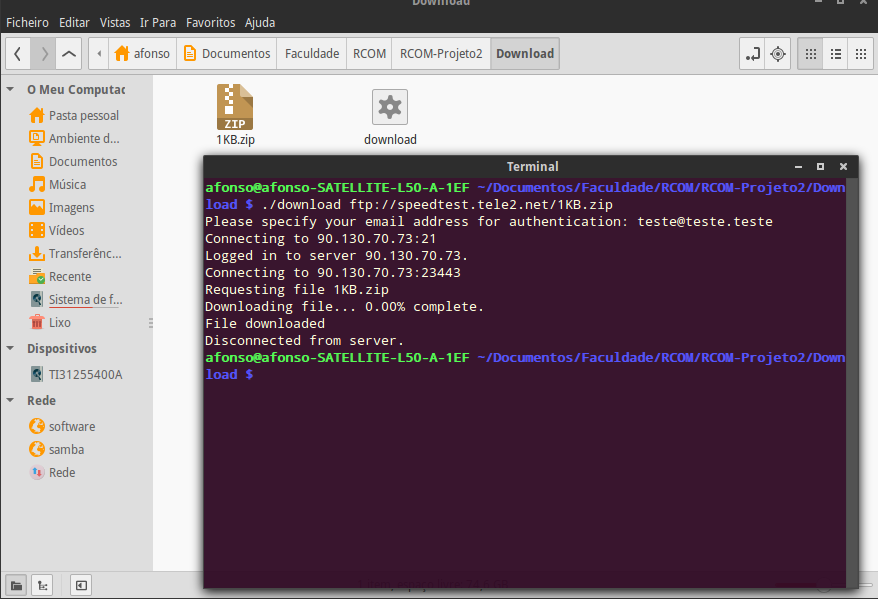
\includegraphics[scale=0.5]{authtest.png}
\caption{Result of the authenticated connection test}
\label{fig:authconnection}
\end{figure}

\begin{figure}[p]
\centering
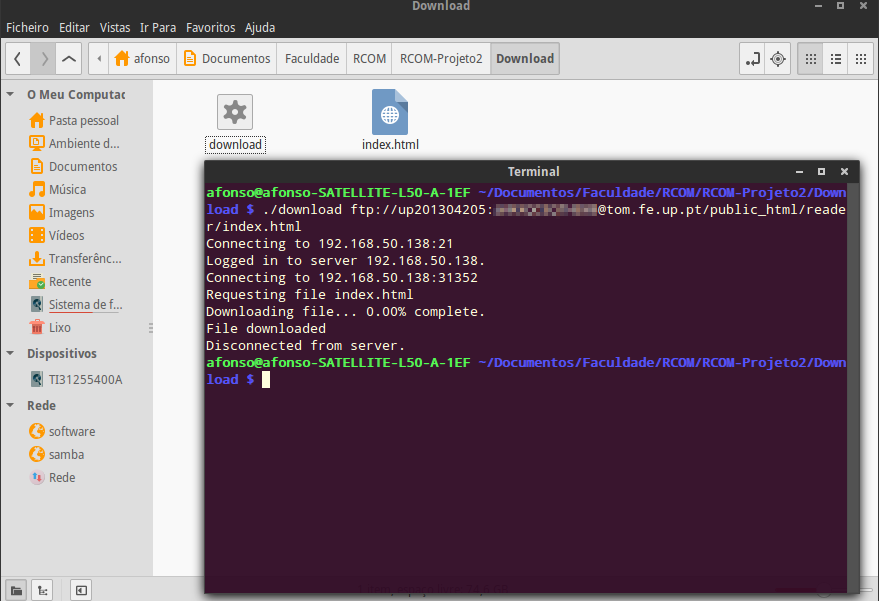
\includegraphics[scale=0.5]{anontest.png}
\caption{Result of the anonymous connection test}
\label{fig:anonconnection}
\end{figure}

\section{Network Configuration and Analysis}

\subsection{Experience 1 - Configure an IP network}

This experience’s objective was to configure a machine network interface IP address and study ARP and ICMP packets. In order to do that Tux1 eth0 interface was assigned the IP adress 172.16.50.1/24 and Tux4 eth0 interface was assigned the IP address 172.16.50.254/24. Both interfaces were connected to the default vlan on the switch (Tux1 eth0 in port Fa 0/1, Tux4 eth0 in port Fa 0/4).

After configuring the network we issued a ping to 172.16.50.254 from Tux1. It generate an ARP packet in order to discover the MAC address whose IP was the requested one. Tux4 replied to Tux1 with its MAC address. After that, an ICMP Echo packet was issued from Tux1 having its MAC and IP as source and having Tux4 MAC and IP as destination. Upon receiving this packet, Tux4 issued an ICMP Echo Reply as response with its MAC and IP as source and Tux1 MAC and IP as destination. By capturing the internet packets navigating through Tux1 eth0 with the Wireshark software we can analyse them in order to inspect their contents and obtain informations such as its ethernet type in the ethernet header, which allows us to distinguish between ARP (0x0806) and IP (0x0800) packects, its IP protocol in the IP header protocol field, which is 1 for ICMP packets, and the length of the receiving frame, which is also in a field of the IP datagram header.

Although it was already configured, the loopback interface is also one of the machine’s network interfaces. It is a virtual network interface that the machine uses to communicate with itself. It is used mainly for diagnostics and troubleshooting, and to connect to servers running on the local machine.


\subsection{Experience 2 - Implement two virtual LANs in a switch}

In this experience with learnt how to setup virtual LANs in a switch and how they affected the communication between the network interfaces connected to the switch.

We began by adding Tux2 eth0 to our setup, assigning it the IP address 172.16.51.1/24 and connecting it to the switch in port Fa 0/2. Then we setup vlan50, added ports Fa 0/1 and Fa 0/4 to it, setup vlan51 and added port Fa 0/2 to it.
After the setup, we used Wireshark and tryed to ping Tux2 and Tux4  from Tux1 but there was no response from Tux2, because Tux2 is not on the same vlan as Tux1 and Tux4.

Next we started Wireshark in all the machines and made a ping broadcast to IP 172.16.50.255 from Tux1. Tux4 replied, but not Tux2. Then we made a ping broadcast to IP 172.16.51.255 from Tux2. This time none of the other machines replied. With this we can conclude that there are 2 broadcast domains.

\subsection{Experience 3 - Configure a router in Linux}

This experience consisted in making one of the Tux machines into a router, connecting the two networks created previously.

For this, tux4 eth1 interface was assigned the IP address 172.16.51.253/24, connected to port Fa 0/5 on the switch and added to vlan51. Then a route was added on tux2 to reach the network 172.16.50.0/24 through gateway 172.16.51.253 and the ip address 172.16.50.254 was assigned as tux1 default gateway.

These configurations allowed communication between the 3 tux machines, which we tested with some ping commands that generated some more ARP,  ICMP Echo and ICMP Echo Reply packets.

Each one of the tux machines as a forwarding table which contains information about a destination network, the gateway to reach it (which is the next hop on the connection), the interface associated with it and a metric, which evaluates the efficiency of a route.
Tux1 has 2 routes on its table: the route to network 172.16.50.0/24, which it has direct access through eth0, and a route to all the other networks with 172.16.50.254 as the gateway, making it tux1 default gateway.

Tux2 has 2 routes on its table: the route to network 172.16.51.0/24, which it has direct access through eth0, and a route to 172.16.50.0/24 with 172.16.51.253 as the gateway.

Tux3 also has 2 routes on its table: the route to network 172.16.50.0/24, which it has direct access through eth0, and the route throught 172.16.51.0/24, which it has direct access through eth1.

When pinging tux2 from tux1, the packet traveling in 172.16.50.0/24 has source IP and MAC address corresponding to tux1 eth0 but, although its destination IP address is tux2 eth0’s IP address, the MAC address is tux4 eth0’s IP address. This packet is then received by tux4 which forwards it to tux2, but it changes the source MAC to tux4 eth1’s MAC and the destination MAC to tux2 eth0’s MAC. A similar operation happens with packets travelling to tux1 from tux2, as expected.

\subsection{Experience 4 - Configure a Commercial Router and Implement NAT}

In order to do so, the router gigabitethernet 0/0 interface was assigned IP address 172.16.51.254/24 and was connected to the switch port Gi 0/1, which was added to vlan51. Then router gigabitethernet 0/1 interface was assigned IP address 172.16.1.59/24 and connected to the lab network. After that we made 172.16.51.254 the default gateway for tux4 and tux2 and added a route on the router for network 172.16.50.0/24 using 172.16.51.253 as the gateway. With these configurations we were able to ping all the network interfaces of tux4, tux2 and the router from tux1.

To analyse route redirections we disabled the acceptance of route redirections on tux2 and removed the route to the network 172.16.50.0/24. Then we used the traceroute utility to check the path taken to 172.16.50.1, which was: tux2, router, tux4, tux1. After restoring the route the path became: tux2, tux4, tux1. By removing again the route but accepting redirects on tux2, the path followed by the first communication was: tux2, router, tux4, tux1 but the following ones were: tux2, tux4, tux1 because the ICMP Redirect packet sent by the router was accepted by tux2, which then started using this more efficient route to network 172.16.50.0/24 than the one it knew.

In the end, we enabled NAT on the router, making the gigabitethernet 0/1 the interface connected to the inside network and the gigabitethernet 0/2 the one conneted to the outside network and allowing access to the networks 172.16.50.0/24 and 172.16.51.0/24. This allowed us to communicate with machines outside our local network through their IP address by translating a machine local IP address to a public IP address by mapping its datagrams IP address and port to a port on the device making the translation and them making the translation backwards when receiving and answer.

\subsection{Experience 5 - DNS}

This experience was centered around using a DNS to access other machines by its domain names. To do that we set IP address 172.16.1.1 as the nameserver for each of the Tux machines.

After that we sent some pings to a domain name. Before issuing the ICMP Echo packet the machine sent an UDP packet with a DNS query to 172.16.1.1 asking for the IP address corresponding to the domain name, which was sent by the nameserver as an answer.

\subsection{Experience 6 - TCP Connection}

In this experience we tested our ftp download application on the network we were configuring.

We started by running it in tux1 and were able to download the requested file, which led us to conclude that both the download application and the network were well configured.

The download application opens 2 TCP connections, one connected to the ftp server port 21 to send the control information and another one connected to the data port provided by the server. These TCP connections are divided in 3 phases: the connection establishement, which is a 3-way handshake, the data transfer, in which the connection data is transmitted, and the connection termination, which is a 4-way handshake. When transfering the data the TCP connetions relies on the a variation of the Go-Back-N ARQ mechanism in order to maintain the integrity of the transmited data. The TCP datagram contains a sequence number field, an acknowledgment number field and an window size field, which are needed to use this ARQ mechanism. In order to achieve a high and stable throughput, the TCP connection has a congestion control mechanism based on ACK’s received, which increase additively the throughput, and timeouts occured, which decrease multiplicatively the throughput.

In the end we opened two instances of the download application, one on tux1 and another on tux2, and analysed the impact of it in the throughput of the connection on tux1. We concluded that the throughput diminished almost to half, as expected.

\section{Conclusion}

After concluding this project, the group considers they understood all the topics asked and managed to solve all the problems proposed, both from the FTP application part and the network configuration and analysis part. All group elements consider they've understood the basics of implementing a computer network, and we had no trouble developing the application and studying the RFC's needed to develop it. 

We'd like to thank our teacher for helping us several times during our classes. Without that support, this project would have been much more difficult to complete, especially some key concepts of the computer network part.

All in all, we all consider the group's objectives were successfully completed.

\newpage

\begin{appendices}

%%%%%%%%%%%%%%%%%%%%%%%%%%%
% APENDICE - CODIGO FONTE %
%%%%%%%%%%%%%%%%%%%%%%%%%%%
\section{Application Source code}

\begin{Large}
ftpClient.c:
\end{Large}

\lstinputlisting[language=C, breaklines=true]{ftpClient.c}

\vspace{15mm}

\begin{Large}
ftpClient.h:
\end{Large}

\lstinputlisting[language=C, breaklines=true]{ftpClient.h}

\vspace{15mm}

\begin{Large}
parseURL.c:
\end{Large}

\lstinputlisting[language=C, breaklines=true]{parseURL.c}

\vspace{15mm}

\begin{Large}
parseURL.h:
\end{Large}

\lstinputlisting[language=C, breaklines=true]{parseURL.h}

\vspace{15mm}

\begin{Large}
main.c:
\end{Large}

\lstinputlisting[language=C, breaklines=true]{main.c}

\vspace{15mm}

\begin{Large}
Makefile:
\end{Large}

\lstinputlisting{Makefile}

\vspace{15mm}

\section{Configuration commands}

\subsection{Configure an IP network}

On tux1:
\begin{itemize}[label=-]
\item ifconfig eth0 up
\item ifconfig eth0 172.16.50.1/24
\end{itemize}

On tux4:
\begin{itemize}[label=-]
\item ifconfig eth0 up
\item ifconfig eth0 172.16.50.254/24
\end{itemize}

\subsection{Implement two virtual LANs in a switch}

On tux2:
\begin{itemize}[label=-]
\item ifconfig eth0 up
\item ifconfig eth0 172.16.51.1/24
\end{itemize}

On switch:
\begin{itemize}[label=-]
\item configure terminal
\item vlan 50
\item exit
\item vlan 51
\item exit
\item interface fastethernet 0/1
\item switchport mode access
\item switchport access vlan 50
\item exit
\item interface fastethernet 0/2
\item switchport mode access
\item switchport access vlan 51
\item exit
\item interface fastethernet 0/4
\item switchport mode access
\item switchport access vlan 50
\item exit
\item end
\end{itemize}

\subsection{Configure a router in Linux}

On tux1:
\begin{itemize}[label=-]
\item route add default gw 172.16.50.254
\end{itemize}

On tux2:

\begin{itemize}[label=-]
\item route add -net 172.16.50.0/24 gw 172.16.51.253
\end{itemize}

On tux4:

\begin{itemize}[label=-]
\item ifconfig eth1 up
\item ifconfig eth1 172.16.51.253/24
\item echo 1 > /proc/sys/net/ipv4/ip\textunderscore forward
\item echo 0 > /proc/sys/net/ipv4/icmp\textunderscore echo\textunderscore ignore\textunderscore broadcasts
\end{itemize}

On switch:

\begin{itemize}[label=-]
\item configure terminal
\item interface fastethernet 0/5
\item switchport mode access
\item switchport access vlan 51
\item exit
\item end
\end{itemize}

\subsection{Configure a router in Linux}

On tux2 and tux4:

\begin{itemize}[label=-]
\item route add default gw 172.16.51.254
\end{itemize}

On switch:

\begin{itemize}[label=-]
\item configure terminal
\item interface gigabitethernet 0/1
\item switchport mode access
\item switchport access vlan 51
\item exit
\item end
\end{itemize}

On router:

\begin{itemize}[label=-]
\item configure terminal
\item interface gigabitEthernet 0/0
\item ip address 172.16.51.254 255.255.255.0
\item no shutdown
\item ip nat inside
\item exit
\item interface gigabitEthernet 0/1
\item ip address 172.16.1.59 255.255.255.0
\item no shutdown
\item ip nat outside
\item exit
\item ip nat pool ovrld 172.16.1.59 172.16.1.59 prefix 24
\item ip nat inside source list 1 pool ovrld overload
\item access-list 1 permit 172.16.50.0 0.0.0.255
\item access-list 1 permit 172.16.51.0 0.0.0.255
\item ip route 0.0.0.0 0.0.0.0 172.16.1.254
\item ip route 172.16.50.0 255.255.255.0 172.16.51.253
\item end
\end{itemize}

Disable tux2 redirection acceptance:

\begin{itemize}[label=-]
\item echo 0 > /proc/sys/net/ipv4/conf/eth0/accept\textunderscore redirects
\item echo 0 > /proc/sys/net/ipv4/conf/all/accept\textunderscore redirects 
\end{itemize}

Enable tux2 redirection acceptance:

\begin{itemize}[label=-]
\item echo 1 > /proc/sys/net/ipv4/conf/eth0/accept\textunderscore redirects
\item echo 1 > /proc/sys/net/ipv4/conf/all/accept\textunderscore redirects
\end{itemize}

\subsection{DNS}

On tux1, tux2 and tux4 replace /etc/resolv.conf with:

\begin{itemize}[label=-]
\item search netlab.fe.up.pt
\item nameserver 172.16.1.1
\end{itemize}


\end{appendices}

\end{document}
